% vim: ft=tex
\chapter{Scope}
This chapter outlines the general scope of this project, beginning with the
students' motivation to work on this bachelor thesis.

The \autoref{sec:scope:init} introduces mindclue GmbH and its Roadster
framework in its state prior to this bachelor thesis to provide the reader with
an understanding detailed enough to comprehend the contributions described in
\autoref{ch:approach}.

Finally, \autoref{sec:scope:goals} elucidates the goals from the original task description
(\autoref{ch:task-desc}), as well as in retrospect.

\section{Motivation}
\subsection{Backgrounds}
To better understand our motivation, it might help to understand our personal
backgrounds first.

\textbf{Patrik Wenger} did his apprenticeship in computer science at Swisscom
Schweiz AG, and stayed work as a full-time employee for five more years
afterwards. In programming he is most fluent in \gls{ruby} and \gls{c}. During
winter 2015/2016, he created \gls{cztop} in leisure time because
there was no suitable Ruby binding for \gls{zmq}/\gls{czmq} available and a side
project of his demanded it. Fascinated with event-driven programming and
software design patterns such as the \gls{actor-model} (e.g. the
Celluloid\footnote{A concurrency framework for Ruby based on the actor model,
\url{https://github.com/celluloid/celluloid}} library on Ruby,
and the Pony programming language\footnote{A young programming language completely based on actors,
\url{http://www.ponylang.org}}), distributed computing and high availability
have long been part of his core interests, especially in conjunction with the
brilliant \zmq library. Having a strong interest in information security and modern
cryptography\footnote{I.e. \gls{nacl} or \gls{libsodium} as used by
\gls{zmq}}, especially in this post-Snowden era, this bachelor thesis could not
be a better match.

\textbf{Manuel Schuler} did his apprenticeship in computer science at
Alcatel-Lucent AG.  Most of his projects involved network monitoring or
configuration automation. In programming he is most fluent in Node.js, Java and .NET. He
made several projects to keep his life simple. After working full-time for
several companies after his apprenticeship, he decided to start his own
business.  Always keen on learning new things and the fact that his work
involved similiar technologies, he did not hestiate to join this bachelor theis
at the first opportunity.

In essence, both students are thrilled to gain more experience in the following
fields and technologies:

\begin{itemize}
	\item Distributed computing
	\item High availability
	\item Information security
	\item \gls{actor-model}
	\item \gls{zmq}
	\item \gls{ruby}
\end{itemize}

\subsection{Opportunities}
Coming from different backgrounds and having different levels of experience in
each of the aforementioned technologies, we cannot wait to learn more about them and put
them to actual use. The fact that the product of this bachelor thesis is most
likely going to be used in the real world only adds to the excitement.

This bachelor thesis involves working with Ruby, the Actor Model, \zmq,
distributed computing with high availability, and state-of-the-art
cryptography. Furthermore, in case of successful completion of this thesis, the results will be used in real-world settings like the Ceneri
Base Tunnel. It is a huge opportunity for a solution completely based on free
and open-source software interacting with other industrial systems over open standards. The students, as well as the client, strongly believe
in customized solutions built on reusable, free open-source software.

In addition to that, we look at this bachelor thesis as an opportunity to
become more fluent in English, both written and spoken, as well as to improve
our skills in crafting scientific documents using {\LaTeX}.

Depending on how we perform together as a team, further collaboration might
result in the future, either between the students themselves, or between the
students and the client. Even if our paths will part, this project will
serve as a valuable reference for future job hunting.

\subsection{Open-source engagement}
Getting the chance to use \gls{cztop} and watch it perform definitely adds to
the motivation as well. Its software design has yet to be proven in more
productive settings.

Another personal goal is to create a reusable open-source library as a
byproduct. The intention is that the library makes certain \zmq-based
communication protocols readily available for other developers facing the same
problems.

\section{Initial situation}\label{sec:scope:init}

\subsection{mindclue GmbH}
The company mindclue GmbH, located in Ziegelbr\"ucke GL, provides its partner
REMTEC AG with complete \gls{SCADA}\footnote{SCADA software resides in level 2 of the enterprise levels (0--4) modeled by the \gls{isa95} standard, \url{https://en.wikipedia.org/wiki/Enterprise_control}} applications. These are then used to
supervise and control operation and safety equipment found in:
% ISA95 “levels”

\begin{itemize}
\item National freeways, e.g. emergency phones
\item Tunnels, e.g. lights, ventilation, and railway electricity
\item Water supply systems
\item Energy facilities
\item Other specialized fields
\end{itemize}

To build these customized applications, their in-house creation
Roadster is used.

\subsection{Roadster framework}
Roadster is a SCADA framework written in Ruby. It has been developed to
produce next-generation SCADA applications to replace legacy
solutions based on its predecessor found in numerous tunnel
facilities in Switzerland.

A Roadster installation combines the following responsibilities:

\begin{itemize}
	\item Interaction with subordinate field devices (monitoring \& controlling)
	\item Sophisticated alarm case management
	\item Persisting data (e.g. time series of sensor data, alarm log)
	\item A machine-to-machine interface to higher level systems (\emph{clients})
	\item A modern web UI customized for the particular installation to interact with operational and executive personnel
\end{itemize}

Among others, the field devices include various kinds of \glspl{PLC}\footnote{E.g.
the SIMATIC S7-1500 by Siemens AG,
\url{http://w3.siemens.com/mcms/programmable-logic-controller/en/advanced-controller/s7-1500/Pages/default.aspx}}
as well as emergency call systems\footnote{E.g. the NIS ComNode by Trans Data
Management AG,
\url{http://trans-data.com/en/k2-categories/item/149-niscomnode}}.
These are interacted with over numerous propietary and standardized protocols,
for which Roadster provides spezialized adapters.

The following two subsections elaborate more on Roadster and how it's used.
However, as far as this bachelor thesis goes, it's not important information
and thus can be skipped.

\subsubsection{System integration}\label{sec:scope:sys-integration}
This section briefly describes the big picture of Roadster's place within
typical production environments and its relationship with other systems.

In some deployments, Roadster has no higher-level client systems, but is
operated as a standalone supervision and control system. In that case, the only
clients would be its human users. This usually applies to solutions delivered
to counties as opposed to solutions operating on a national level.

In other deployments, there are higher level systems which act as clients of a Roadster instance, communicating over
protocols including \gls{SOAP} and \gls{opc-ua}. Their purpose is to
collect and aggregate supervisory data from larger regions. At the top of the
hiearchy are the \gls{FEDRO} (German: \gls{ASTRA}) which combine the information of all
subsystems to provide a nationwide overview.

\begin{figure}[]
	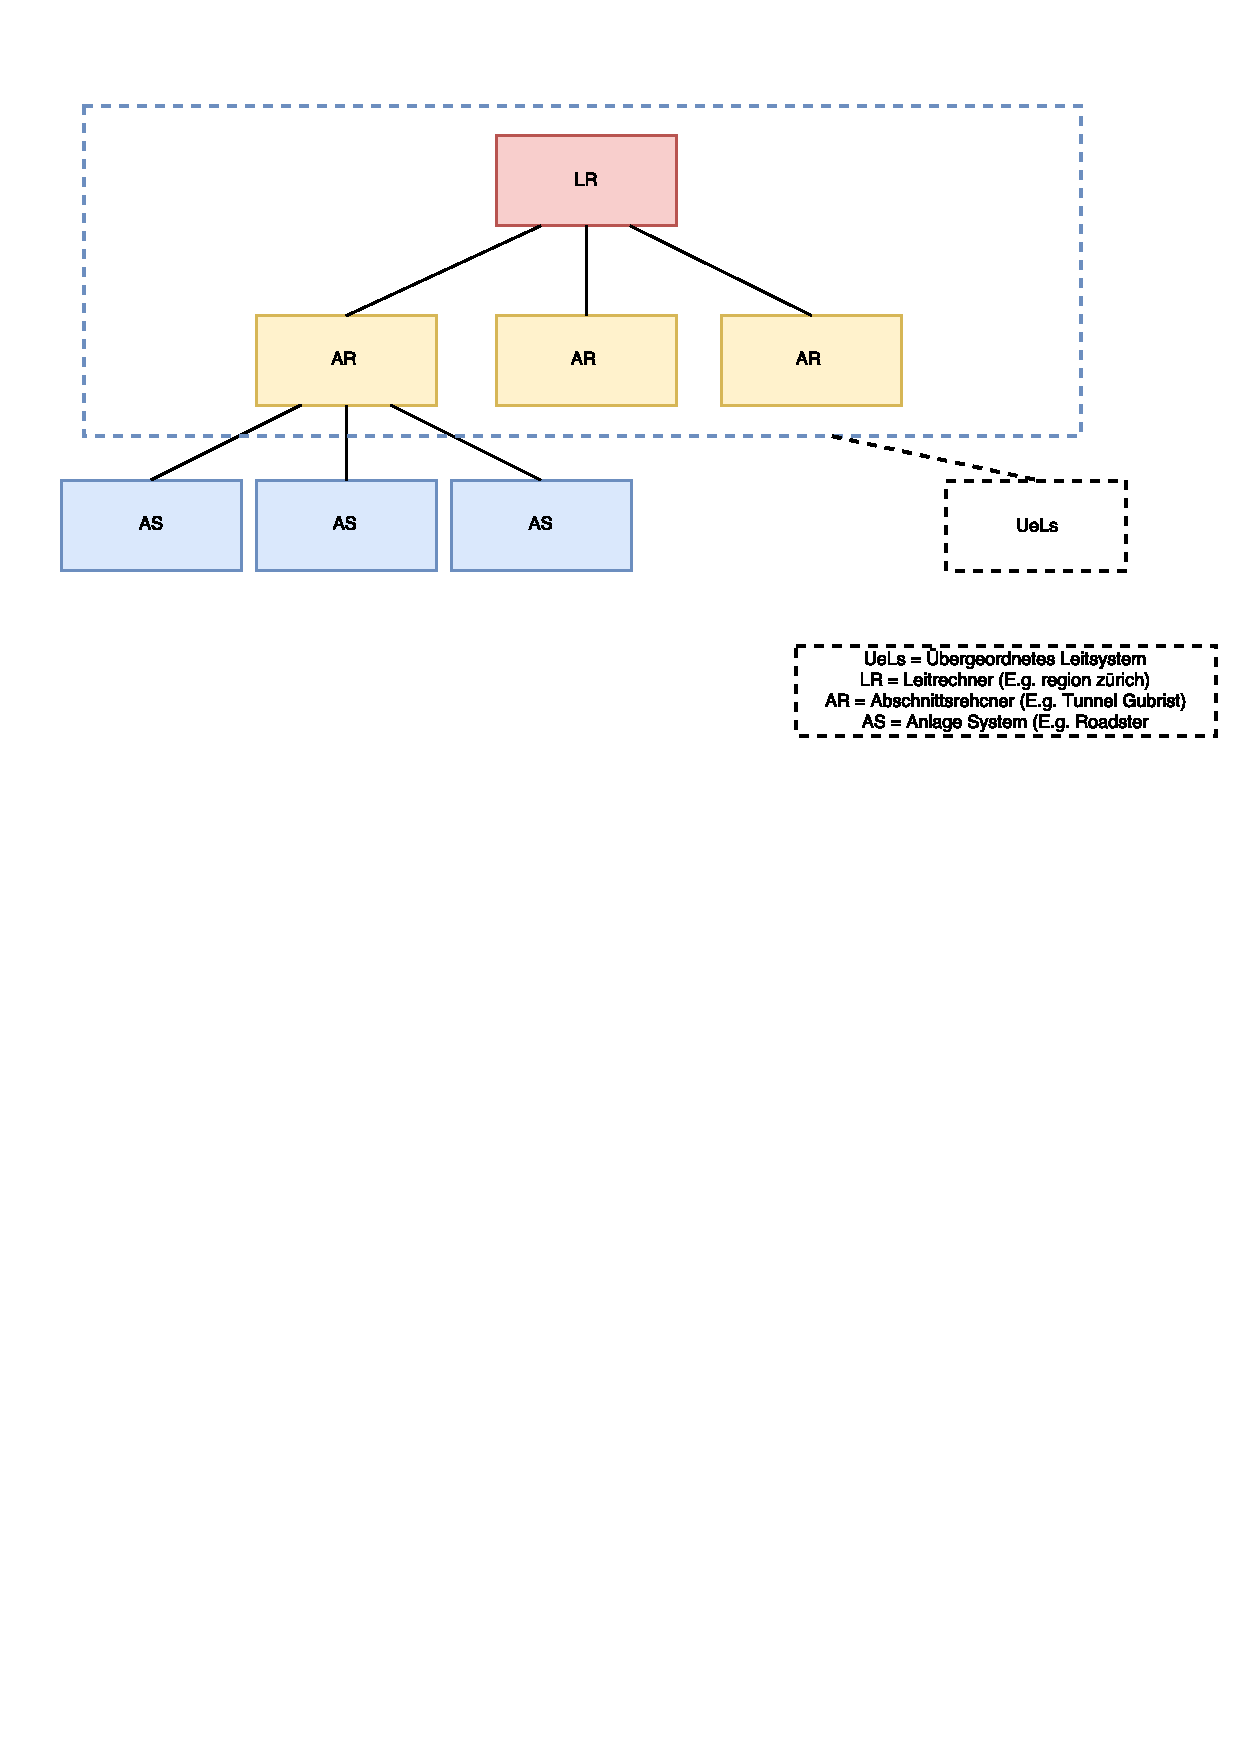
\includegraphics[width=\textwidth]{img/overall_system.pdf}
	\caption{Roadster's place within a typical system}
	\label{fig:roadster:overallsys}
\end{figure}

\autoref{fig:roadster:overallsys} illustrates the typical system. The acronyms
used, which are part of the \gls{FEDRO} terminology, do not have official
English translations; not even the department itself was able to help with
translations on request, so they were left unchanged. A brief description
follows, from the bottom up:

\begin{description}
	\item [ Field devices: ] \hfill\\
	Field devices are various kinds of \glspl{PLC} and other subordinate systems
	used to supervise and control industrial processes. Communication with them
	happens over protocols such as \gls{modbus-tcp}, \gls{iec-104}, and
	\gls{opc-ua}.

	\item [ \gls{AS}: ] \hfill\\
	This is Roadster's domain, or, of course, the domain of another product with similar
	functionality. An AS is responsible for one facility (e.g. emergency call system,
	lighting system, fire alarm system, video monitoring system, ventilation
	system, power supply system, train signaling system).

	\item [ \gls{AR}: ] \hfill\\
	The higher level system of the collection of all AS found in one larger
	facility such as a tunnel. With the results of this bachelor thesis, this
	\emph{could} be Roadster's domain as well.

	\item [ \gls{LR}: ] \hfill\\
	The higher level system of the collection of all AR found in a region such as
	Z\"urich. As with AR, this \emph{could} be Roadster's domain as well.

	\item [ \gls{LTA}: ] \hfill\\
	This collective term comprises both the levels of AR and LR. For
	simplicity and readability's sake, this will be referred to as
	\emph{client} for the remainder of this document.
\end{description}

\subsubsection{Typical hardware}
Roadster typically runs on entry-level rack server hardware powered by an
Intel\textregistered{} Xeon\textregistered{} processor, or industrial box PCs for smaller systems
commonly used for \gls{IoT} which are powered by more energy efficient processors
such as Intel\textregistered{} Core\textregistered{} and Intel\textregistered{}
Atom\texttrademark{}. The machines are usually equipped with 4 -- 6 GiB of main
memory and Gigabit Ethernet. For reliable systems without any moving parts, an
industrial grade \gls{SSD} or two (in a software \gls{RAID} level 1 setup) are used.


\subsection{Software architecture}
As mentioned earlier, Roadster is \gls{event-driven} and built on the Actor model, meaning it exhibits a
\gls{shared-nothing-arch}. Each Roadster node runs a number of Ruby processes
which communicate via \zmq sockets. The key here is communication:

\begin{quote}
``Don't communicate by sharing state; share state by communicating.''
\end{quote}

Running multiple, loosely coupled processes (actors) allows leveraging the full
potential of modern multi-core processors, while avoiding a whole class of
concurrency issues present in traditional concurrency models based on shared
memory and synchronization constructs such as semaphores.

Every Roadster node runs a group of actors:

\begin{description}
	\item [CORE:]\hfill\\
		The CORE actor is responsible to maintain aggregates of supervisory data
		(e.g. sensor data) and create alarm cases to inform
		about critical situations.

		During the application startup it is responsible to start the
		other actors and later on routes messages between them. It also
		plays a key role in keeping state in all actors synchronized. More
		about that in \autoref{sec:scope:csp}.

	\item [COMM:]\hfill\\
		COMM actors communicate with the external services accessible
		by a node. Each of them employs a specific communication
		protocol to act as an adapter to one of various field devices
		(usually called \emph{peers}), or as a server to an attached client
		system.\\

		The exact set of COMM actors running on a particular
		installation depends on a configuration file available to the
		installation.\\

		The webserver for the web UI is one of the COMM actors, denoted
		by COMM.WEBUI.

	\item [STORAGE:]\hfill\\
		This actor is used when information needs to be persisted, such
		as time series or event journals. It is the interface to a
		key-value store.

	\item [LOGGER:]\hfill\\
		This actor collects logging data and sends it to whatever
		target is configured, be it \gls{stdout}, a file, or a syslog server.

	\item [CONSOLE:]\hfill\\
		This actor is not fully implemented yet. It's supposed to
		be a textbased user interface for maintenance and trouble shooting.
\end{description}

\autoref{fig:roadster:arch} illustrates Roadster's architecture. The red boxes
with arrows attached to the actors represend the \zmq sockets which are used
for inter-actor communication. More information about \zmq sockets in
\autoref{sec:scope:zmq}.

\begin{figure}[]
	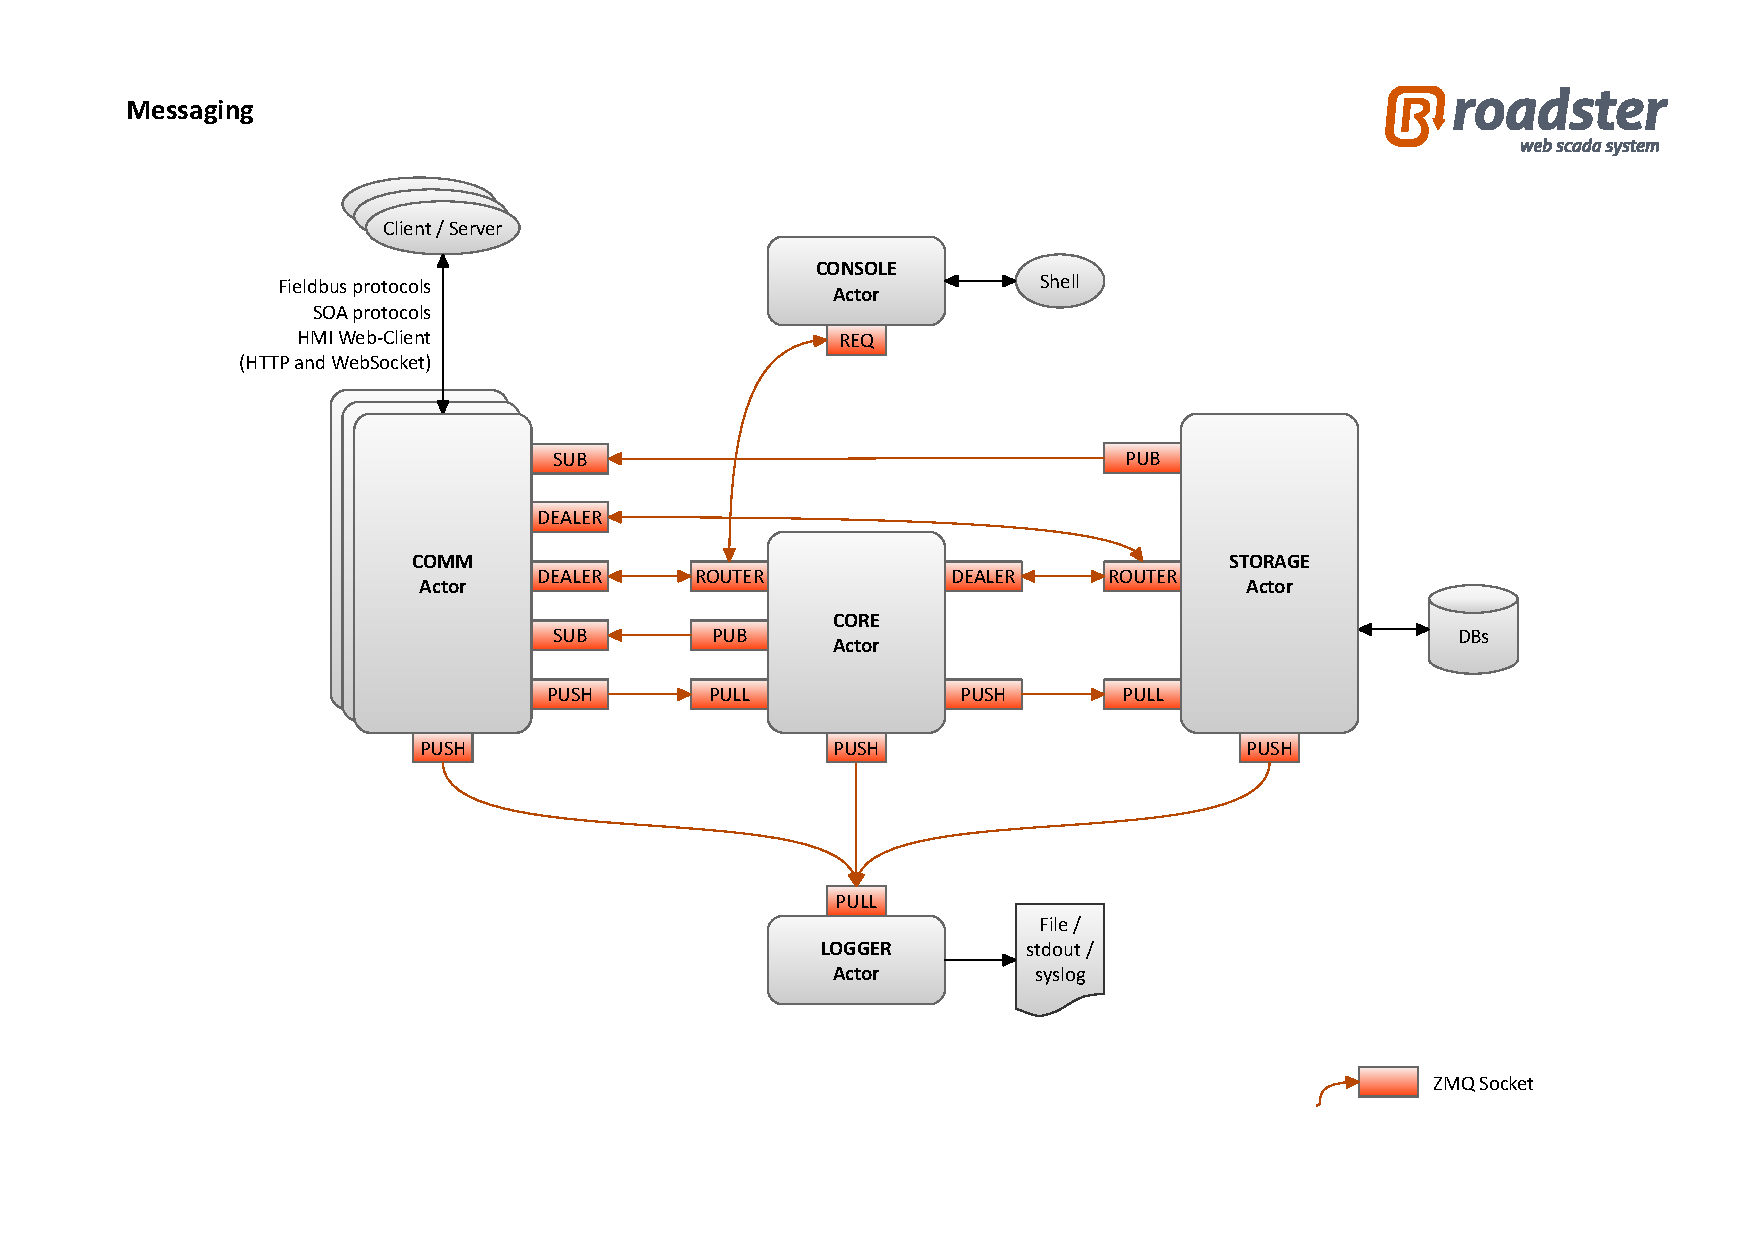
\includegraphics[trim=4cm 2cm 3.5cm 2.8cm, clip=true, width=\textwidth]{img/roadster_arch.pdf}
	\source{mindclue GmbH}
	\caption{Roadster's software architecture}
	\label{fig:roadster:arch}
\end{figure}

Each actor of Roadster employs three abstraction layers
as illustrated in \autoref{fig:roadster:layers}.  The following
list briefly explains the layers from top (most abstracted) to bottom:

\begin{description}
	\item [Engine layer:]\hfill\\
		Here is the business logic of Roadster, e.g. the \gls{DIM},
		user authentication, adapters for external devices, the web
		\gls{UI}, etc.

	\item [Messaging layer:]\hfill\\
		The \gls{RMP} reside here and implement essential protocols used
		for logging, state synchronization, commands, application controlling,
		and storage. They're explained later in \autoref{sec:rmp}.

	\item [Reactor layer:]\hfill\\
		This layer forms the base, which is where the \zmq sockets and
		\glspl{websocket} are utilized. It is powered by an
		event-loop\footnote{EventMachine is used as a high-performance event-loop to
		manage large numbers of sockets and timers,
		\url{https://github.com/eventmachine/eventmachine}}. Sockets used by COMM actors
		to communicate with various field devices are also integrated into this
		event-loop.

\end{description}

Following the reactor design pattern, the event-loop informs Roadster about
data received on sockets (i.e. \zmq messages or other protocol data), which is
then read and processed using the upper two layers in the next event
tick. This approach eliminates most concurrency issues because within an actor,
nothing actually happens in parallel. An actor merely reacts on messages and
timers sequentially.

\begin{figure}[]
	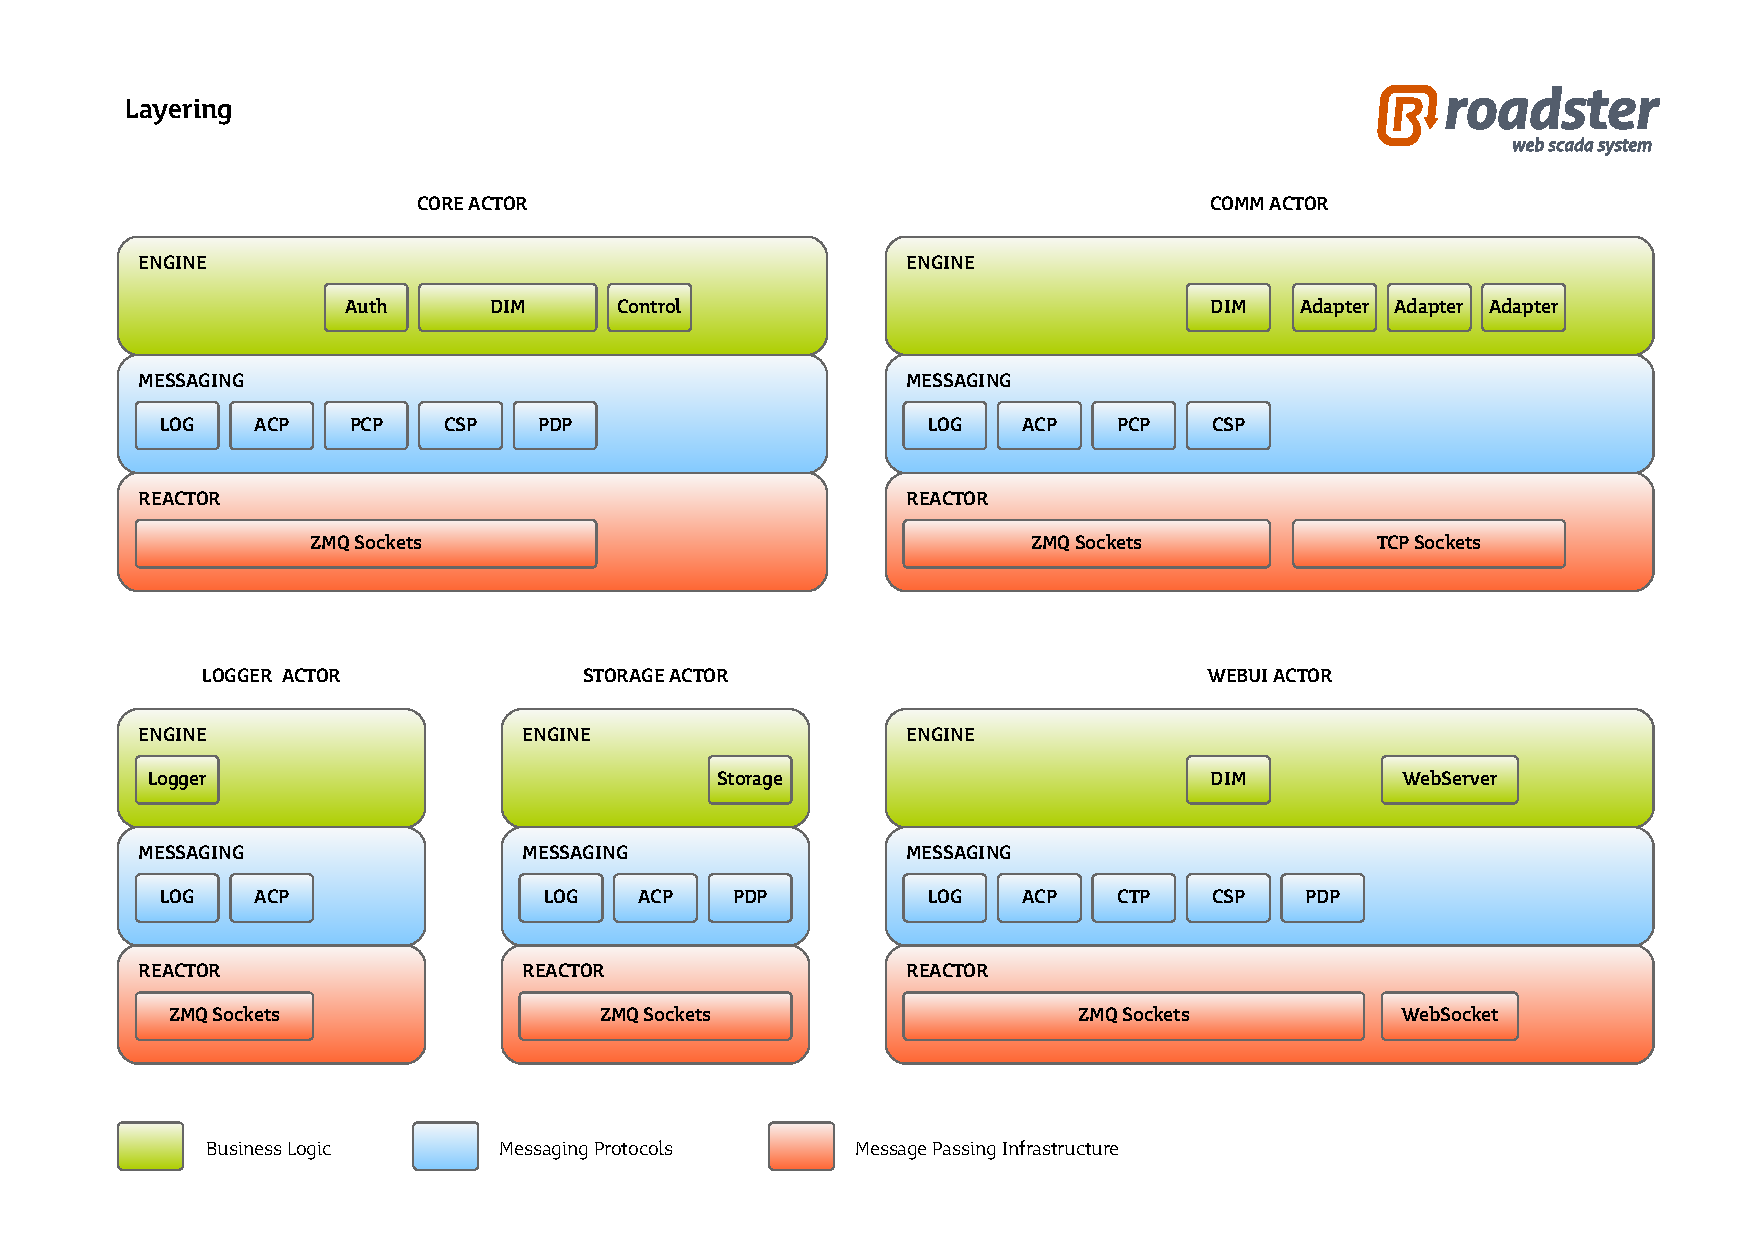
\includegraphics[trim=1.95cm 2.5cm 1.65cm 2.8cm, clip=true, width=\textwidth]{img/roadster_layering.pdf}
	\source{mindclue GmbH}
	\caption{Roadster's communication layers}
	\label{fig:roadster:layers}
\end{figure}


\subsection{Domain Informaton Model}
The \acrfull{DIM} is a tree data structure that is maintained by every actor
taking part the in business logic of a Roadster node, which are all but the LOG
and STORAGE actors.  The CORE actor and every COMM actor build the DIM from the
installation's configuration files\footnote{The configuration is written in a
\gls{DSL} defined as part of the model classes of Roadster. Ruby makes it easy
to define concise, expressive DSLs.} when starting up. The resulting collection
of domain model instances commonly counts up to a few hundred objects,
depending on the attached field devices and configuration items.


\autoref{lst:roadster:dim-tree} shows the hierarchical structure of a
DIM comprising about 60 objects (shortened to increase readability), including:
\begin{itemize}
	\item Access control lists (users, roles, authentication and authorization rules)
	\item Navigation menus and pages for the web UI
	\item An adapter for a robot field device (utilized by a COMM actor) and its peer, the robot
	\item \emph{Variables} and \emph{aggregates} based on the robot's current position
	\item A guard for the robot
\end{itemize}

The purpose of guards (instances of \sh{Roadster::Domain::Model::Guard}) is to
observe certain variables and aggregates for changes. In case a sensor value
exceeds the range declared as part of the guard, an alarm case is created,
which requires human interaction.


\autoref{fig:roadster:meta-model} illustrates the class diagram of
all the classes instanciated to constitute the DIM. They are all defined within the
Ruby module namespace \sh{Roadster::Domain::Model}.
Most of these these objects are static, but some are dynamic:
\begin{itemize}
	\item The current value of a \emph{variable} or an \emph{aggregate}, stored in an instance of \\
		\sh{Roadster::Domain::Model::DataItem}
	\item Current sessions of web UI users (\sh{Roadster::Domain::Model::Session})
	\item Pending alarm cases (\sh{Roadster::Domain::Model::Case})
\end{itemize}
Modifications to the dynamic objects are replicated across all DIM-aware
actors, which is performed by the \gls{CSP} as explained in~\autoref{sec:scope:csp}.


\begin{listing}
	\begin{minted}[bgcolor=bg]{Text}
root (Root)
root.navigation (Entity)
root.navigation.home (Page)
root.navigation.home.process (Menu)
# [...] 6 more Menu and Page objects clipped
root.var_map (Entity)
root.access_control (Acl)
root.access_control.users (Entity)
root.access_control.users.admin (User)
# [...] user credentials (Parameters) clipped
root.access_control.users.guest (User)
# [...] user credentials (Parameters) clipped
root.access_control.roles (Entity)
root.access_control.roles.superuser (Role)
# [...] 5 Role and Parameter objects clipped
root.access_control.sessions (Entity)
root.version (Variable)
root.version.datum (DataItem) = 0
root.adapters (Entity)
root.adapters.simu (Adapter)
root.adapters.simu.version (Variable)
root.adapters.simu.version.datum (DataItem) = 0
root.adapters.simu.robot_controller (Peer)
root.adapters.simu.robot_controller.conn_state (Variable)
root.adapters.simu.robot_controller.conn_state.datum (DataItem) = "CONNECTED"
root.objects (Entity)
root.objects.robot (Robot)
root.objects.robot.control_mode (Parameter)
root.objects.robot.control_mode.datum (DataItem) = "AUTO"
root.objects.robot.position_x (Variable)
root.objects.robot.position_x.datum (DataItem) = 30.0
root.objects.robot.position_y (Variable)
root.objects.robot.position_y.datum (DataItem) = -9.0
root.objects.robot.polar_position_radius (Aggregate)
root.objects.robot.polar_position_radius.datum (DataItem) = 31.32092
root.objects.robot.polar_position_radius.alarm_guard (Guard)
root.objects.robot.polar_position_angle (Aggregate)
root.objects.robot.polar_position_angle.datum (DataItem) = -16.69924
  \end{minted}
  \caption{An example list of objects in a DIM}
  \label{lst:roadster:dim-tree}
\end{listing}

\begin{figure}[]
	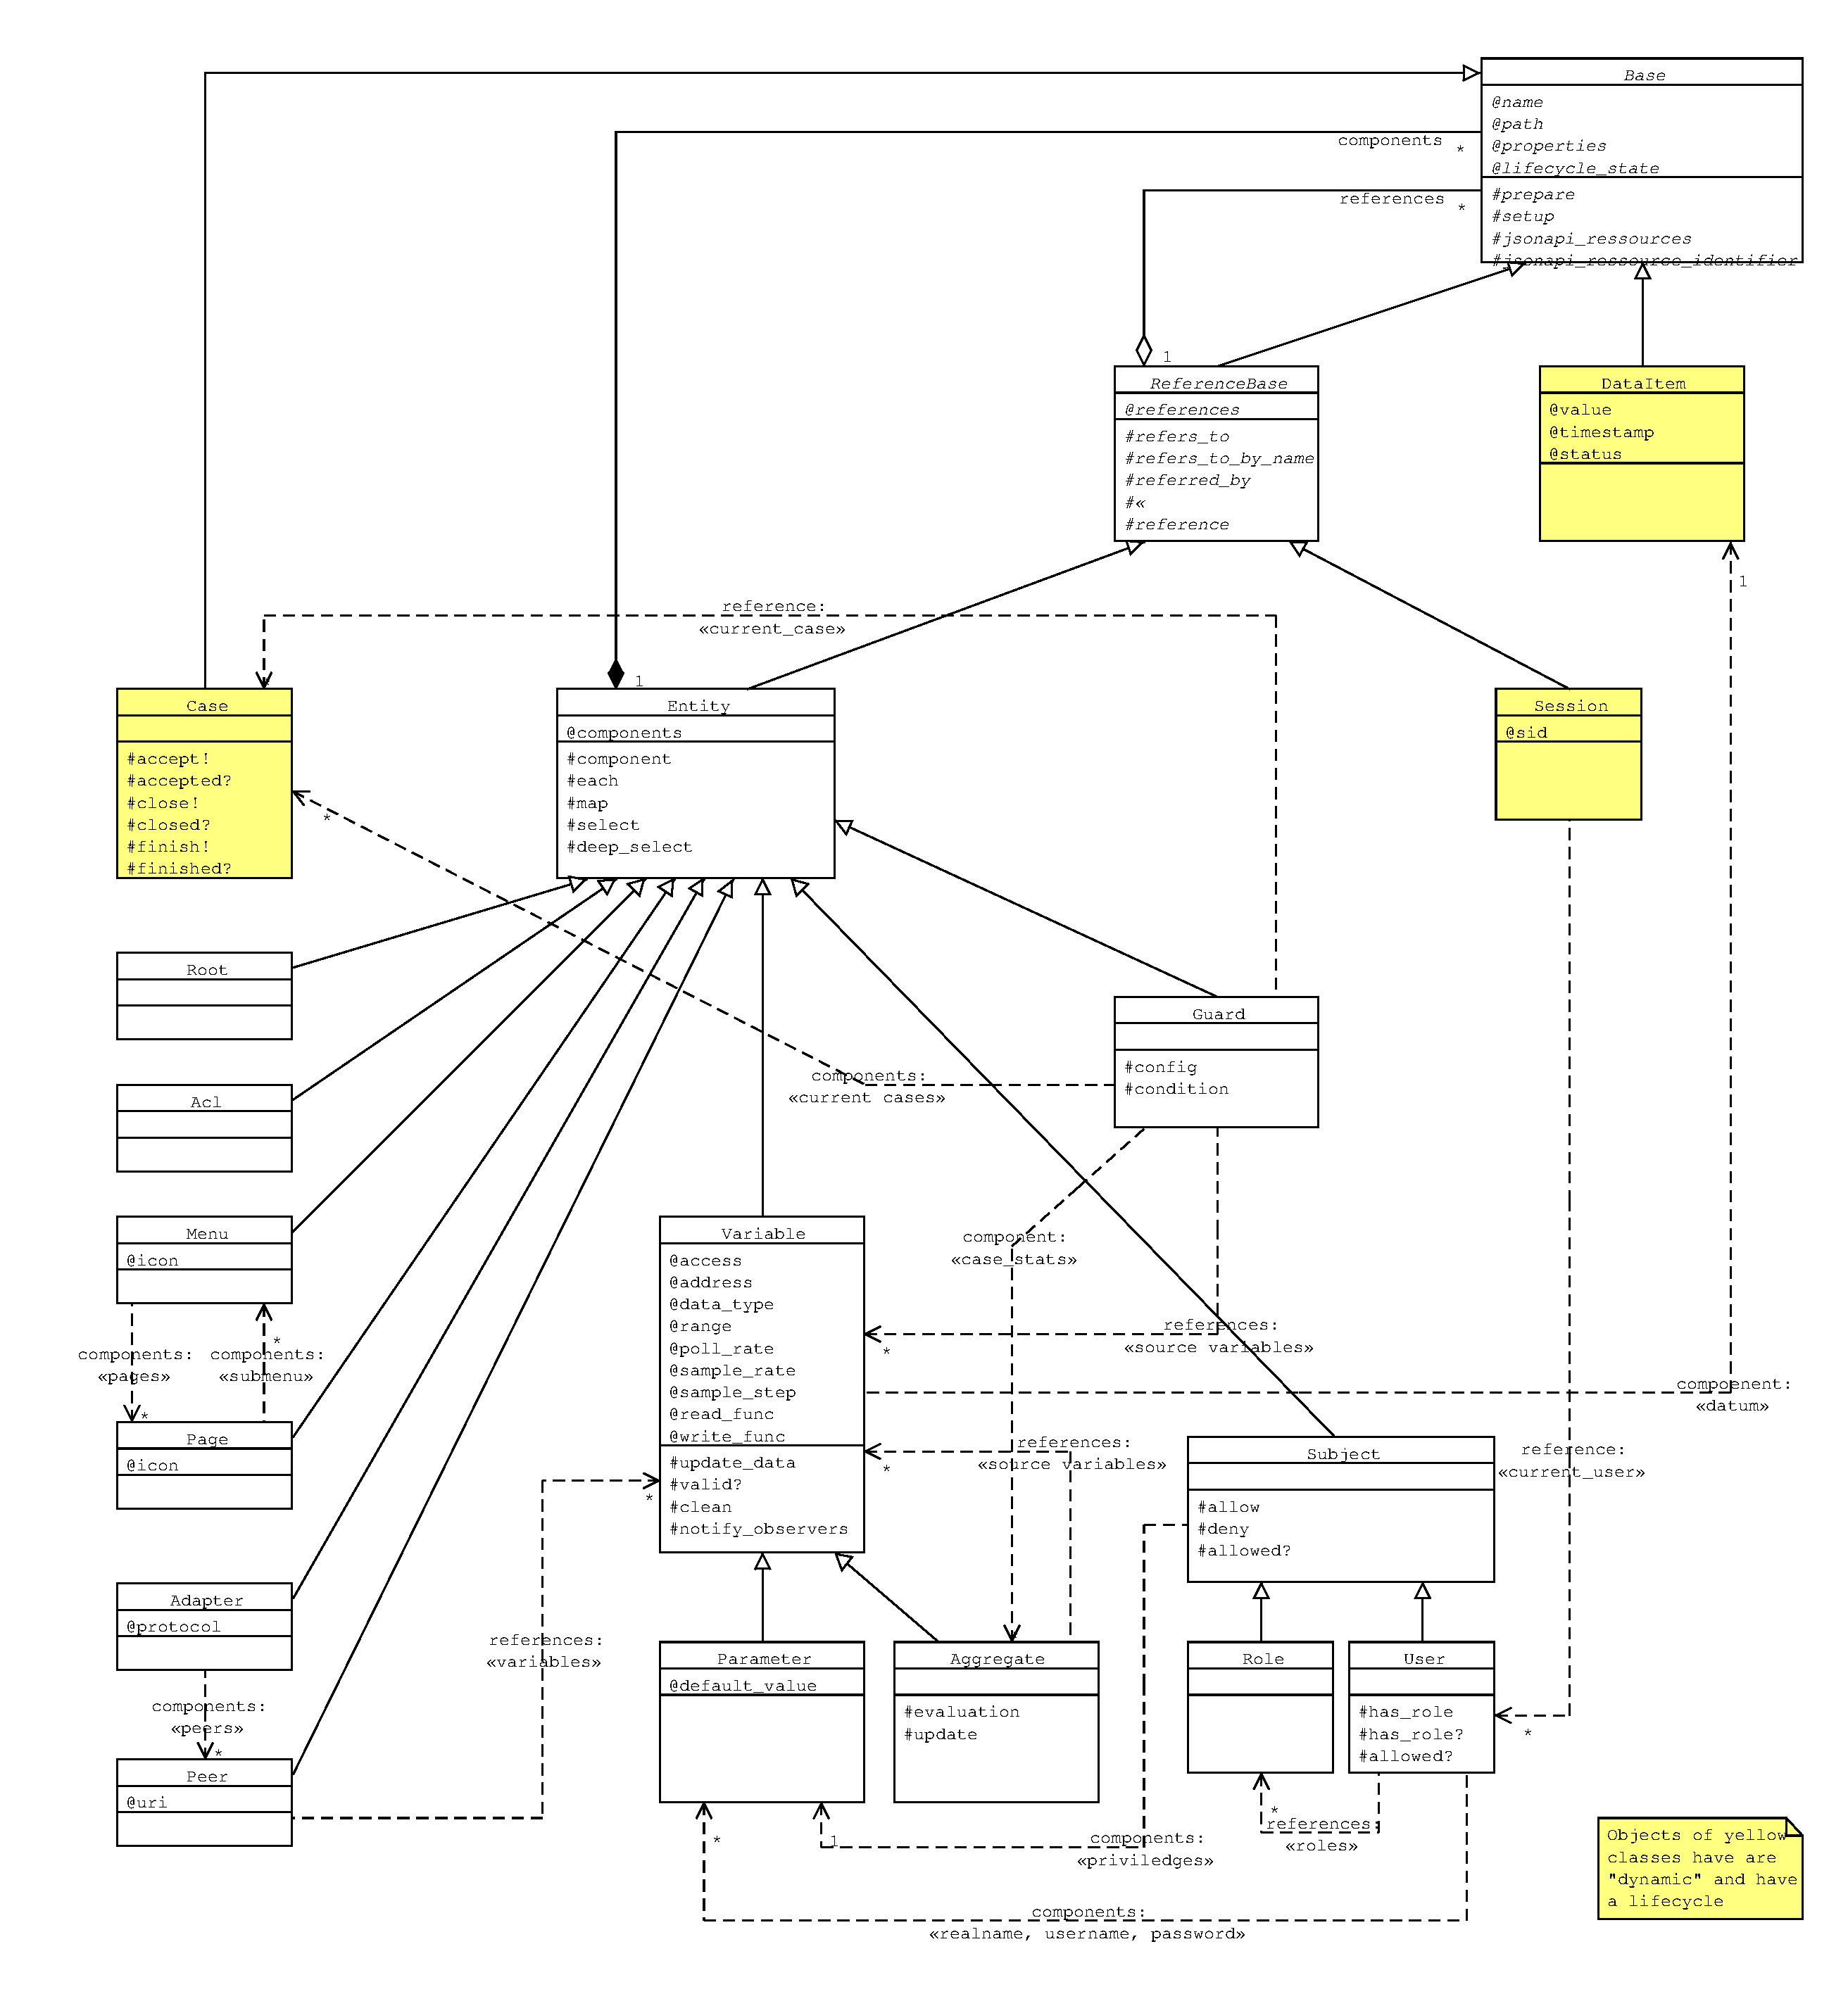
\includegraphics[trim=1.5cm 1cm 1cm 1cm, clip=true, width=0.9\textwidth]{img/meta_model.pdf}
	\source{mindclue GmbH}
	\caption{Class diagram for Roadster's domain model used in the DIM}
	\label{fig:roadster:meta-model}
\end{figure}

\subsection{Roadster Messaging Protocols}\label{sec:rmp}
The \gls{RMP} are a collection of protocols implemented and used by Roadster
internally. They reside in the messaging communication layer, and include:

\begin{description}
	\item [\gls{ACP}:]\hfill\\
		Used to control the application state, e.g. shutdown.
	\item [\gls{CMP}:]\hfill\\
		Used to accept pending \glspl{case}.
	\item [\gls{CSP}:]\hfill\\
		Used to synchronize state between the DIM-aware actors.
	\item [\gls{LOG}:]\hfill\\
		Used for system logging. Log messages from all actors are sent
		to the LOGGER actor via this protocol.
	\item [\gls{PCP}:]\hfill\\
		Used for command execution via COMM peers with feedback.
	\item [\gls{PDP}:]\hfill\\
		Used when data needs to be persisted via the STORAGE actor.
	\item [\gls{SMP}:]\hfill\\
		Used to suppress the generation of certain alarm cases, e.g.
		when a sensor is defect and repeatedly reports critical sensor data.
\end{description}

Each protocol offers \glspl{API} endpoints for the different roles of
participants, a subset of which are then registered in every actor to fulfill
its responsibilities.

The next section provides more detail about the different
delivery guarantees available for message passing.

\subsubsection{Reliability modes}
Following the \gls{actor-model}, messages are passed between actors
asynchronously. This happens in one of two reliability modes:

\begin{description}
\item [Fire \& Forget:]\hfill\\
No guaranteed delivery. This does not mean there are no other mechanisms in
place to ensure reliability, e.g. employed by a protocol itself.\footnote{such
as what \gls{TCP} does by sequencing the segments of a stream}

\item [Dialog:]\hfill\\
An immediate answer is expected, e.g. when creating a user
session. Any protocol can make use of this primitive. Source code that
initiates a dialog looks like a synchronous call, even though
it is handled asynchronously by Roadster's message passing
infrastructure.\footnote{This is done by wrapping the affected
code in a Ruby \sh{Fiber}, which is similar to a thread but
allows for cooperative scheduling as opposed to preemtive.}
\end{description}


\subsection{Directory structure}
\autoref{lst:roadster:directory-structure} gives an annotated overview of Roadster's directory structure.

\begin{listing}
	\begin{minted}[bgcolor=bg]{Text}
roadster
|-- benchmarks                # Benchmark scripts
|-- bin                       # The `roadster` utility
|-- doc                       # Generated API documentation
|-- lib                       # Framework implementation
|   `-- roadster
|       |-- actors            # Reactor layer: Base, Core, Comm, ...
|       |   `-- em-zmq        # Adapter for ZMQ library
|       |-- adapters          # IEC-104, Modbus TCP, OPC, ...
|       |-- engines           # Engine layer: Base, Core, Comm, ...
|       |-- messaging         # Messaging layer: Dialog
|       |   |-- handlers      # Base, Core, Comm, dispatching, ...
|       |   |-- messages
|       |   `-- protocols     # ACP, CMP, CSP, LOG, PCP, PDP, SMP, ...
|       |-- misc              # Conf, Exceptions, Ruby core extensions
|       `-- tools             # CLI
|-- roadster-webui-core
`-- spec                      # Unit and integration tests of the above
    |-- actors
    |   |-- em-zmq
    |-- adapters
    |-- engines
    |-- messaging
    |   |-- handlers
    |   |-- messages
    |   `-- protocols
    `-- support               # Fixtures
        `-- domains
  \end{minted}
  \caption{Directory structure of the Roadster framework}
  \label{lst:roadster:directory-structure}
\end{listing}




\subsection{\zmq}\label{sec:scope:zmq}
As mentioned earlier, Roadster uses \zmq to carry messages between its actors.
To understand the rest of this document, it is
helpful to understand the basics of \zmq. This is a brief introduction to
\zmq for the unfamiliar reader. What follows is a quote from the \gls{zguide}
which does a fairly good job at describing \zmq in a hundred words:

\begin{quote}
``ZeroMQ (also known as \zmq, 0MQ, or zmq) looks like an embeddable networking
library but acts like a concurrency framework. It gives you sockets that carry
atomic messages across various transports like in-process, inter-process, TCP,
and multicast. You can connect sockets N-to-N with patterns like fan-out,
pub-sub, task distribution, and request-reply. It is fast enough to be the
fabric for clustered products. Its asynchronous I/O model gives you scalable
multicore applications, built as asynchronous message-processing tasks. It has
a score of language APIs and runs on most operating systems.  ZeroMQ is from
iMatix and is LGPLv3 open source.''
\end{quote}

\subsubsection{Messages}
A message is just an array of one or more parts (\emph{frames}). From the point
of view of \zmq, each message frame is simply a
chunk of opaque data. Object serialization is outside the scope of \zmq and can be done using
JSON, XML, ASN.1, MessagePack, Google's Protocol Buffers, Apache Thrift, or a
programming language's own implementation of object marshalling, which is what
Roadster does for inter-actor communication. JSON is used between the WEBUI
actor and the actual web application running in the HTTP user agent.

\subsubsection{Socket types}
A number of socket types are provided, of which the most important pairs are:

\begin{description}
	\item [ROUTER and DEALER sockets] \hfil\\
	These sockets implement an asynchronous request-reply communication
	pattern. When sending a message via a DEALER socket, it is sent
	to any of the connected ROUTER sockets (usually just one). When
	reading a message from a ROUTER socket, an additional frame is
	prepended to identify the DEALER socket which sent the message.
	In \zmq terminology, this kind of frame is called an
	\emph{envelope}.
	This identity is a short string (up to 255 bytes) either randomly chosen by \zmq
	or set by the application as a socket option. It does NOT
	resemble an IP address or anything dependent on the chosen
	transport.

	When sending a message via a ROUTER socket, the same
	process happens in reverse: The first frame is taken away and
	used to determine the receiving DEALER socket, which will
	receive all but the first frame.

	Roadster's CORE actor uses a ROUTER socket to send or relay
	messages to specific actors.


	\item [PUSH and PULL sockets] \hfil\\
	These sockets implement an asynchronous pipeline communication pattern
	providing fan-out and fan-in techniques. PUSH sockets can only be
	written to whereas PULL sockets can only be read from.


	Within Roadster, this socket pair is used to perform efficient
	replication of modifications to the DIM. More about CSP
	in~\autoref{sec:scope:csp}.


	\item [PUB and SUB sockets] \hfil\\
	A publish-subscribe communication pattern is provided by these two
	sockets. Message distribution based on subscription to one or
	more topics is possible (simply by matching the beginning of the first
	frame).

	At this point, Roadster actors simply
	subscribe to all messages sent via a the CORE's PUB socket.

\end{description}

Any socket can be either bound and/or connected to any number of endpoints. A few examples:

\begin{itemize}
	\item A simple message passing application following the client-server
		model, can bind a ROUTER socket on the server and connect each
		client's DEALER socket to it. After that, any one of the server
		or the clients can asynchronously send a message.

	\item A SUB socket can connect to multiple PUB sockets to receive
		published messages from all of them

	\item A parallel pipeline can be built using a PUSH socket that fans
		out tasks, which are then read by one of possibly many worker
		instances via its PULL socket.
\end{itemize}

In any of the above cases, the number of connected remote sockets does not
matter. To the application, it's still a single socket, which just happens to
communicate with many other sockets.

\subsubsection{Transport}
The transport technique and transport-specific connection handling is completely
abstracted away by \zmq. There's no possibility that such implementation
details leak into an application which would result in an unwanted increase of
external coupling.

This also means that it does not matter whether an application communicates with
other \zmq sockets within the same process, on the same machine, or on a remote
machine. Common transports are \gls{unix-domain-socket}, \gls{TCP},
\gls{TIPC}, as well as \gls{PGM} based multicast.

\subsubsection{Software packages}
Roadster uses a Ruby gem (software package) called
\emph{ffi-rzmq}\footnote{\url{https://github.com/chuckremes/ffi-rzmq}} to
interface with \zmq. It is unmaintained and does not support newer features of
\zmq (namely secure communication).


For a more details about \zmq, including the \gls{czmq} abstraction layer and
the \gls{cztop} langauge binding for Ruby, see \autoref{ch:zmq}.


\subsection{Existing CSP in a nutshell}\label{sec:scope:csp}
The existing \acrfull{CSP} is closely related to the \gls{clone-pattern} from
the \gls{zguide}. Its goal is to keep the \gls{DIM} (\emph{state}) synchronized
across the set of DIM-aware actors.  It follows a server-client architecture as
opposed to a fully decentralized architecture, which allows for greatly reduced
complexity.

The server part acts as the authorative source for all modifications to the
DIM. This part is performed by the CORE actor and makes use of its ROUTER, PULL, and
PUB socket.

The client part is performed by all COMM actors and utilizes the respective
actor's DEALER, PUSH, and SUB socket.

The protocol consists of three distinct messages flows:

\begin{description}
	\item [Snapshots:]
		Requesting and receiving the complete, current snapshot of the
		state. This is performed via the ROUTER-DEALER pair of sockets
		during the startup of each COMM actor. The CORE actor responds
		with the complete set of dynamic DIM objects.

		In the best case, the snapshot only needs to be requested once
		by each COMM actor. However, as there is no guaranteed message
		delivery, it could happen that an incremental update (issued by
		another COMM actor or the CORE itself) gets lost. With the next
		successfully delivered update, this situation is recognized by
		the receiving COMM actor based on the strictly monotonically
		increasing sequence number (\emph{version}) associated with
		each update. The discrepancy is resolved by simply requesting a
		new snapshot, after which the state has been resynchronized.

	\item [Upstream updates:]
		Updates can originate from a COMM actor (i.e. a new sensor data
		from a field device read by the actor's adapter) and are sent to the
		CORE actor via the PUSH-PULL socket pair.  This works by
		marking the updated objects as ``dirty'' so they can be sweeped
		and marked as ``idle'' when sending the next state update.

		The CORE itself can modify the state as well, i.e. re-evaluate
		aggregates based on changed sensor data, or create/close a
		case. Of course, this change does not need to be sent through a
		PUSH socket first, as it happens directly inside the CORE
		actor. However, the subsequent behavior is the same, namely
		that the new modifications need to be replicated to the other
		COMM actors.

	\item [Downstream updates:]
		After being applied to the CORE's state,
		modifications get a sequence number and are replicated to all
		COMM actors. This happens via the CORE's PUB socket, so all
		COMM actors' SUB sockets receive the update.
\end{description}

By making all updates go through the CORE actor, a single sequence is enforced,
which is crucial to keep the state consistent across all DIM-aware actors.

To avoid risking a gap between requesting the current snapshot and subscribing
to updates, a COMM actor actually subscribes to the updates first, then gets the
snapshot, and then starts reading the updates from the SUB socket (which has been
queueing updates in the meantime, if any). Updates that are older or the same
age as the received snapshot are skipped, and only successive updates are
applied (tested by comparing the sequence numbers).

Because message loss via the third message flow (PUB-SUB) is unlikely but
theoretically possible, the participating actors check for gaps in the sequence number of
each downstream update. If a gap is detected, the current state is discarded and a
complete resynchronization happens. This is brutal, but is very simple and thus
robust; there is no complexity that would leave room for nasty corner cases.

Updates from COMM actors have their own version number, one for each adapter.
This ensures that the CORE is able to do the very same checks to notice
gaps in the sequence of updates from any COMM actor.

% TODO: mention subtrees somewhere else, maybe in the approach
%A feature described in the \gls{zguide}, but not implemented in Roadster as of
%this writing, are subtrees.
%Keys can be treated hierarchically (e.g. \sh{topic.subtopic.key}) and thus, a
%client can optionally subscribe to only a particular subtree. This is useful
%when the number of client grows and not all of the state needs to be on every
%client. In that case, the topic of interest is sent by the client along with
%the ICANHAZ message.

% TODO: add illustration

\subsection{Persistence}\label{sec:scope:persistence}
Certain data on a Roadster node is persisted, which is done by the STORAGE
actor. It uses the
\gls{tc} library as a
serverless key-value store, similar to what the more commonly known
SQLite\footnote{\url{https://www.sqlite.org}} library provides for relational data.

A rough estimation from mindclue GmbH states that, according to data retention
policies, the long-term accumulated data of a Roadster node can be up to $\sim$300 MiB.

There are three kinds of persisted data which are stored in different database files:

\begin{description}
	\item [ Event journal: ] \hfill\\
		The event journal is a history of all \glspl{case}, including the ones
		that have been confirmed and thus removed from the DIM. It
		resides in a \gls{tc} \emph{table} database, where the key is a
		\acrshort{UUID}, one of the columns (attributes) is the timestamp of
		the case, and another one is the actual, serialized \sh{Case}
		object. Objects in this database can be modified, e.g. when a
		pending case is confimed.

	\item [ Time series: ] \hfill\\
		This is a pure key-value store that stores samples of sensor
		data from field devices. Only the most recent value of these
		are actually kept in the DIM. One file per series is used. The
		timestamp is part of the key.

	\item [ Parameters: ] \hfill\\
		Parameters are the third and last kind of persisted data in
		Roadster. Parameters are typically changed by a user. Each
		parameter is backed by a default value from the configuration,
		which is used as long as there is no actual corresponding value
		set or read from the database. Examples include credentials for
		users of the web UI.
\end{description}


\subsection{Tests}
Roadster comes with a few unit tests, and a number of integration tests,
written in RSpec, a well known \gls{BDD} framework for Ruby projects. Test coverage is
about 67\% overall, some files being better covered, some files less. There are
no system tests.

\section{Goals}\label{sec:scope:goals}
To summarize the mandatory goals from the task description in \autoref{ch:task-desc}:

\begin{enumerate}
	\item Getting familiar with Roadster
	\item Extending the communication protocols to support federation of
		multiple nodes
	\item Extending the communication protocols to allow high availability
		clusters of two peer nodes
\end{enumerate}

The optional goals are:

\begin{enumerate}
	\item Encryption of the communication
	\item Providing of the highly available \gls{opc-ua} server interface
\end{enumerate}


\subsection{In retrospect}
During the Elaboration phase when gathering requirements (\autoref{ch:reqs})
and implementing prototypes (\autoref{sec:approach:prototypes} in \autoref{ch:approach}), the
aforementioned goals developed into the following more concrete tasks
(documentation tasks excluded):

\begin{enumerate}
	\item Get familiar with Roadster, especially its multilayer software architecture
	\item Port Roadster onto a new \zmq binding
	\item Provide the ability to declare a federation of Roadster nodes
	\item Inter-node messaging
	\item Heartbeating between a supernode and its subnodes
	\item Message routing to arbitrary nodes in the federation
	\item Creation of alarm cases when a neighboring node is unresponsive
	\item Provide the ability to declare a HA node's primary and backup endpoints
	\item Correctly start engines on two HA peers (going either active or passive)
	\item Selection of the correct supernode (if it's a HA node), which could trigger a failover
	\item Correctly recognize the situation where the passive HA peer needs
		to promote itself to the new active peer
	\item Correctly activate engines on the passive node during failover
	\item Creation of an alarm case when one of the HA peers becomes unresponsive
	\item Reliably replicate persisted data to the supernode
	\item Secure the communication on inter-node sockets using authenticated encryption
	\item Restrict secure communication to selected neighbors based on their public keys
	\item Perform message authentication to ensure end-to-end security (not
		only hop-by-hop which is encompassed by the previous goal)
	\item Provide the ability to declare a node's public key
	\item Provide an utility to generate a new private key
	\item Provide infrastructure so client system interfaces can also trigger a failover
\end{enumerate}


\subsection{Additional goals}
The goals described in this section are neither explicitly, nor implicitly part
of the original task description, but developed out of personal interest in the
technical matter.

\subsubsection{Security concerns of SCADA applications}
Secure inter-node communication within a Roadster federation is important to
mitigate common security concerns with SCADA systems which are becoming more
and more open due to standardization. To quote \cite[Security issues]{wp:scada}
wikipedia:

\begin{quote}
``In particular, security researchers are concerned about:
	\begin{itemize}
		\item the lack of concern about security and authentication in
			the design, deployment and operation of some existing
			SCADA networks
		\item the belief that SCADA systems have the benefit of
			security through obscurity through the use of
			specialized protocols and proprietary interfaces
		\item the belief that SCADA networks are secure because they
			are physically secured
		\item the belief that SCADA networks are secure because they
			are disconnected from the Internet.''
	\end{itemize}
\end{quote}

The goal is to provide a framework that makes it trivial to provide reasonably
secure SCADA applications which are assumed to be running on insecure networks.

\subsubsection{Fallacies of distributed computing}
At this place, it is worth noting the common fallacies encountered in
distributed computing, as explained on \cite{dcomp:fallacies}.

\begin{description}
	\item [The network is reliable.] \hfill\\
		Network outages need to be embraced and handled with
		appropriate error-handling to avoid stalls, permanent
		resource consumption, and the need for manual restarts.

	\item [Latency is zero.] \hfill\\
		The ignorance of network latency and packet loss can lead to
		wasted bandwidth when traffic is unbounded. Depending on the
		application, assuming instant packet delivery could lead to
		timing issues like hanging user interfaces, especially if some
		nodes are not in the same LAN.

	\item [Bandwidth is infinite.] \hfill\\
		Trying to send too much information can lead to bottlenecks,
		slow applications, and simply wasted bandwidth.

	\item [The network is secure.] \hfill\\
		This touches the subject mentioned before. SCADA applications
		often run in isolated networks, at least not directly reachable
		from the internet, but that does not make them secure. Threats
		from within are real and thus one cannot assume a network is
		secure.

	\item [Topology does not change.] \hfill\\
		Topology changes constantly. Services are added and removed. An
		application must not depend on specific endpoints or routes.

	\item [There is one administrator.] \hfill\\
		The overhead introduced by having coordinate multiple
		administrators is not negligible and can constrain one's options
		when e.g. having to upgrade software.

	\item [Transport cost is zero.] \hfill\\
		Getting application entities onto the wire costs, i.e.
		computational resources and in some cases money. Data needs to
		be serialized, which takes CPU cycles and adds to the latency.
		Network equipment to e.g. mitigate the other fallacies -- e.g.
		to make it (more) reliable and more secure -- can cost more
		money than is planned for in the project budget.

	\item [The network is homogeneous.] \hfill\\
		Virtually all networks include devices running different
		operating systems, in different versions, on different
		hardware. On an application level, different subsystems are
		implemented in different programming languages or speak
		different protocols.

\end{description}

The goal is to conduct this thesis with the aforementioned fallacies in mind and embrace
them in the resulting contributions.
